%!TEX root = ../report.tex
\chapter{Introduction}
\label{cha:Introduction}

In computer science, graphs are structures sed for representing relationships between objects. A graph consists of vertices connected by edges, where the vertices represent the objects, and the edges represents the relationship. A graph can take on different shapes, giving the graph special properties. By giving the edges a direction the graph can take on further properties.

When using graphs as a form of storage, the vertices hold the data, and the edges are given an extra property describing the relation. Combining such a data store with common traversal methods for graphs results in an efficient extraction model for relational data. Comparing graph storage to relational storage, such as SQL, graph storage generally outperforms relational storage on structural queries, but not on data queries \cite{AComparisonOfGraphAndRelDB}.

Using standardized models such as the Resource Description Framework (RDF), which is created specifically for graph based data, have made the distribution of graph data easier. One pard of RDF describes so called triples. A triple is a description of nodes, and the connection, using the structure ``subject-predicate-object''. In this structure the subject and object can be considered vertices, and the predicate is the edge. In addition to forming the relation between the two vertices, the predicate also holds a type of relation. This makes it possible to apply reason to the data set, and derive new information from what is already there.

There are few applications using RDF as an information storage system. Some of the more well known are DBPedia\cite{dbpedia}, YAGO\cite{yago}, and Creative Commons. These applications often consists of a large linked data set, or in the case of Creative Commons, it is used for embedding licenses. Creating methods that allows for easy access to information in RDF data makes it possible to create applications with utility. In this thesis methods for efficient keyword search on spatial and temporal data will be explored.

\begin{figure}[h]
    \centering
    \includegraphics[scale=0.5]{figs/SimpleGraph.png}
    \caption{Simple Directed graphs.}
    \label{fig:DAG}
\end{figure}

\begin{figure}[h]
    \centering
    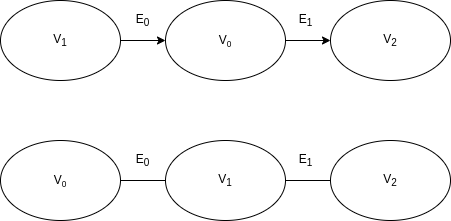
\includegraphics[scale=0.5]{figs/DAGvsAG.png}
    \caption{Example of Directed an non-directed graphs.}
    \label{fig:DAGvsAG}
\end{figure}

\begin{figure}[h]
    \centering
    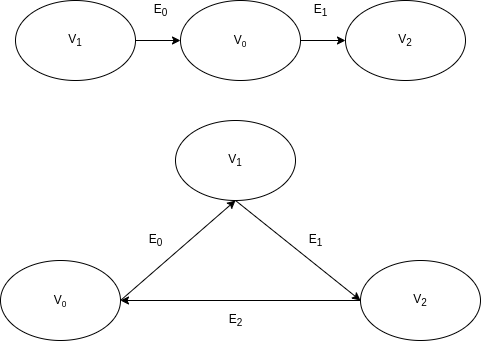
\includegraphics[scale=0.5]{figs/DAGvsDG}
    \caption{Directed graph with and without cycles.}
    \label{fig:DAGvsDG}
\end{figure}


\section{Background and Motivation}
\label{sec:BackgroundAndMotivation}
Traditionally relationships between pieces of data have been difficult for computers to model. Regular SQL databases requires expensive joining to be able to display relationships between entities. As more data is generated, there are also more relations between the data. Exploring these relations can be done by using RDF or other graphs, but for a regular person this can be difficult. By proving that fast and accurate keyword search of spatiotemporal RDF graphs is possible new utilities for exploration can be built.


\section{Goals and Research Questions}
\label{sec:Goals and Research Questions}
\begin{description}
    \item[Goal] {\em With this thesis the goal is to determine if and how spatiotemporal keyword searching in large scale RDF graphs is possible to do in fast and accurate.}
\end{description}
% Why this goal
Accomplishing this goal proves that RDF graphs can be used as a tool for structuring data related to real world places. There is a lot of data that can be placed at one or more real locations, either directly, or indirectly. By using RDF graphs it is possible to model how different places are connected through some pice of data, and how different pieces data can be related to real places.

\begin{description}
    \item[Research question 1] {\em How can spatiotemporal data be integrated into exiting keyword query methods for RDF data.}
\end{description}

\begin{description}
    \item[Research question 2] {\em What methods can be used to create more effective queries on RDF data.}
\end{description}

\begin{description}
    \item[Research question 3] {\em How do spatial and temporal RDF query methods differ from from other query methods.}
\end{description}

\section{Research Method}
\label{sec:researchMethod}
This thesis will build on previous keyword search approaches for RDF graphs, and determine what methods can be expanded to incorporate spatiotemporal queries. A method for spatiotemporal search will be created, and methods for improvement will be tested, with the goal of finding what aspects of the search method have most effect for speed and accuracy.

% \section{Thesis Structure}
% \label{sec:thesisStructure}

\glsresetall